
\section{Rappels}

\begin{frame} \frametitle{Le modèle de données Cassandra}

  Cassandra organise les données en \alert{tables} dénormalisées

  \vfill

  Principales différences avec le modèle relationnel

  \vfill
  \begin{redbullet}
  \item Pas de clé étrangère (et pas de jointure)
  \item Imbrication (\textit{nesting}) de valeurs structurées
  \item Pas d'indépendance logique/physique\,: la clé
      détermine le placement
  \end{redbullet}

  \vfill

  \begin{defblock}{Principe de conception}
  Pas de jointure, donc pas de symétrie d'accès\,: on doit organiser
  les données en fonction des accès applicatifs.

  \end{defblock}
\end{frame}


\begin{frame}[fragile] \frametitle{Structure d'un schéma}

\begin{columns}
    \begin{column}{0.45\textwidth}
  
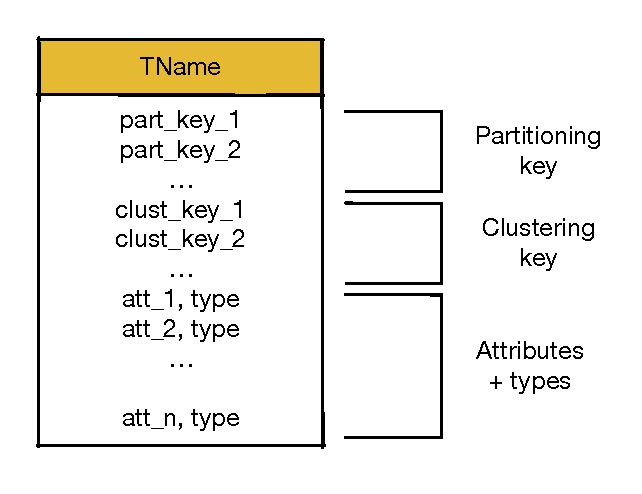
\includegraphics[height=.8\textwidth]{../figures/cassandra_chebotko.pdf}
  \end{column}
 \begin{column}{0.45\textwidth}
 \begin{minted}{sql}
 create table Tname (
   part_key_1 type,
   part_key_2 type,
   ... type,
   clust_key_1 type,
   ... type,
   att_1 type,
   att_2 type,
   ... type,
   primary key ( 
       (part_key_1, part_key2, ...), 
       (clust_key_1, clust_key_2, ...) 
       )
 )
 \end{minted}
\end{column}
\end{columns}

\end{frame}

\begin{frame}[fragile]
\frametitle{Imbrication de structures}

C'est le principe de dénormalisation\,: on regroupe 
les données le plus possible dans des lignes pour éviter les jointures.

\vfill

Un attribut  attribut peut correspondre\,:
\begin{redbullet}
	\item à un ensemble de valeurs (non ordonnées)\,: \textbf{SET} 
	\item à une liste de valeurs \textbf{LIST}
	\item à un dictionnaire\,: \textbf{MAP} 
	\item à un tuple\,: \textbf{TUPLE} 
	\item à une instance d'un type utilisateur
\end{redbullet}

\end{frame}

\begin{frame}[fragile] \frametitle{Clé de partitionnement = placement}

\begin{columns}
    \begin{column}{0.45\textwidth}
  
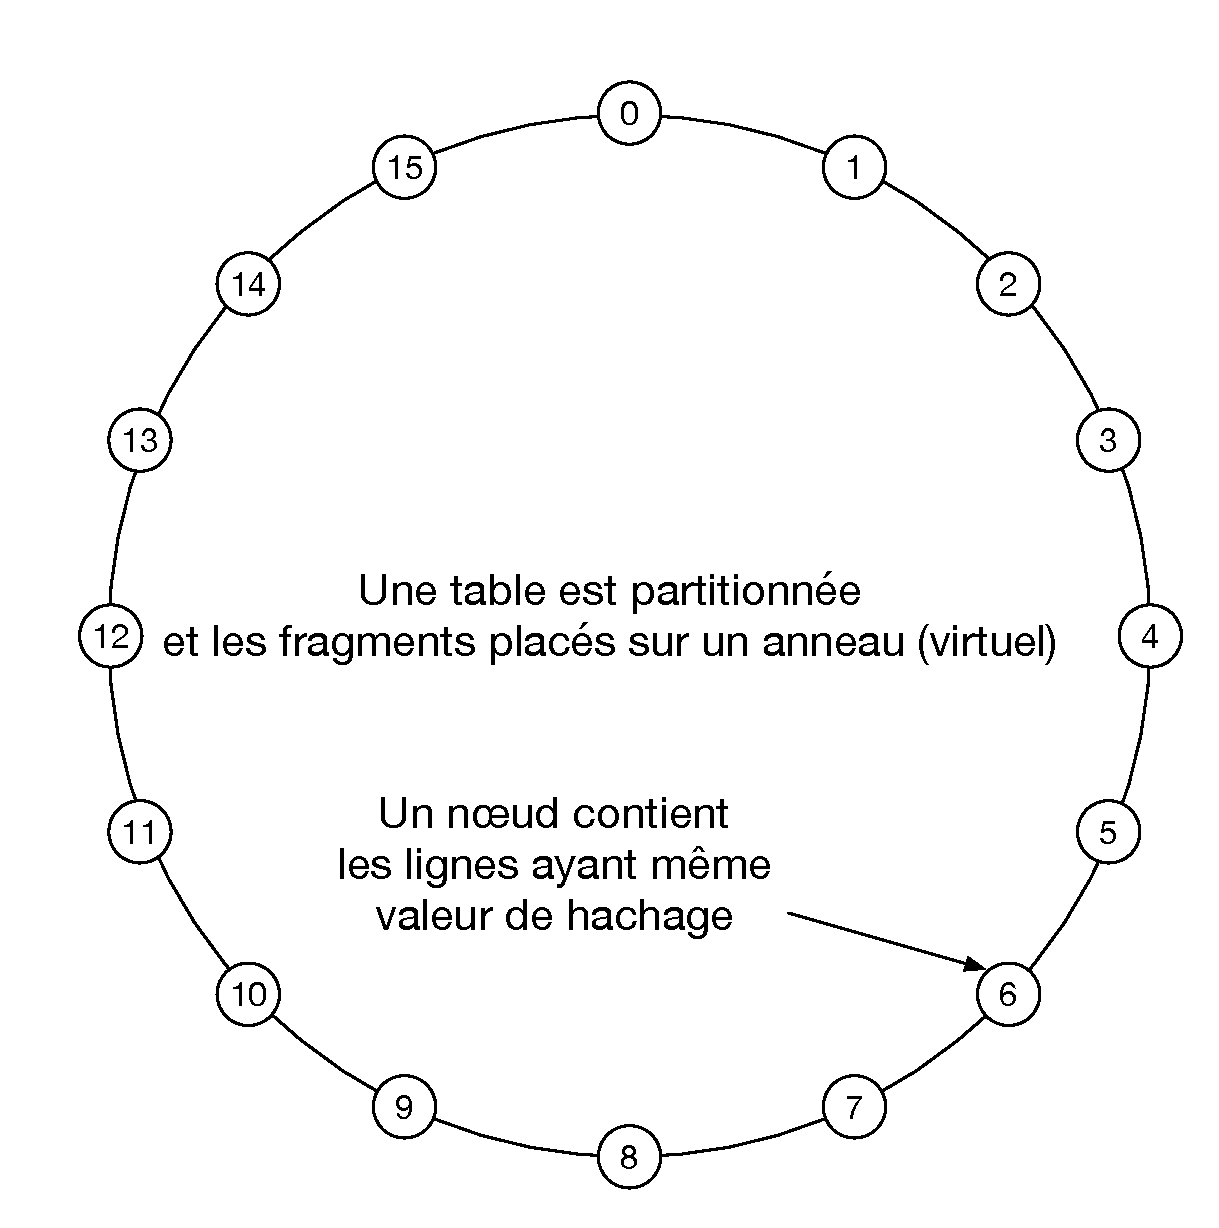
\includegraphics[height=\textwidth]{../figures/cassandra_anneau.pdf}
  \end{column}
 \begin{column}{0.45\textwidth}
\begin{redbullet}
		\item Pour chaque ligne on applique une fonction de hachage 
		          aux valeurs de la clé de partitionnement
		\item La valeur de hachage détermine le placement dans le système distribué
		\item $\Rightarrow$ une requête avec comme critère une clé de partitionnement
		     ne concerne qu'un seul serveur
	\end{redbullet}

\end{column}
\end{columns}

\end{frame}

%%%%%%%%%%
\begin{frame}[fragile] \frametitle{Clé de regroupement = contiguité}

\begin{columns}
    \begin{column}{0.45\textwidth}
    
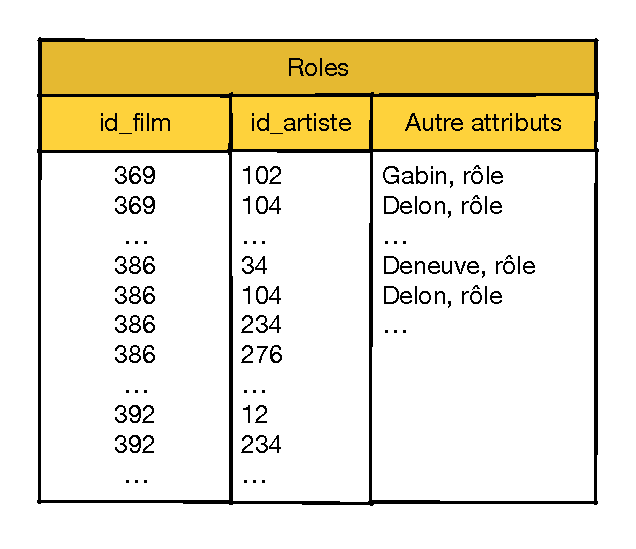
\includegraphics[height=\textwidth]{../figures/cassandra_clustering.pdf}
  
  \end{column}
 \begin{column}{0.45\textwidth}
\begin{redbullet}
		\item Dans un fragment (sur un serveur) les lignes sont triées 
		sur la clé primaire
		\item Pour une même valeur de partitionnement,  les lignes 
		   sont \alert{consécutives} et ordonnées sur la clé de regroupement
		\item $\Rightarrow$ une requête sur une préfix de la clé 
		    primaire (part. + regroupement)
		     correspond à un parcours \alert{séquentiel} sur un seul nœud
	\end{redbullet}

\end{column}
\end{columns}

\end{frame}

%%%%%%%%%%%
\begin{frame}[fragile] \frametitle{Principes de conception}

Très différent du relationnel. On adopte un des nombreux choix possible en 
fonction des besoins supposés.

\vfill

\begin{redbullet}
		\item On conçoit les \alert{chemins d'accès}, ou séquence des requêtes émises par une application
		
		\item On organise les tables pour que  chaque requête  s'exécute \alert{localement} et \alert{séquentiellement}
		
		\item On peut créer ponctuellement des index ou des vues matérialisées
		
		\item Au pire (mais inévitable\,?) on multiplie les organisations physiques et donc la redondance
	\end{redbullet}

\vfill

\begin{defblock}{Pour quelle type d'application\,?}
Acceptable pour une approche WORM (\textit{Write Once, Read many})
\end{defblock}
\end{frame}


%%%%%%%%%%%%%%
\begin{frame}[fragile]{Notre modèle}

\begin{center}
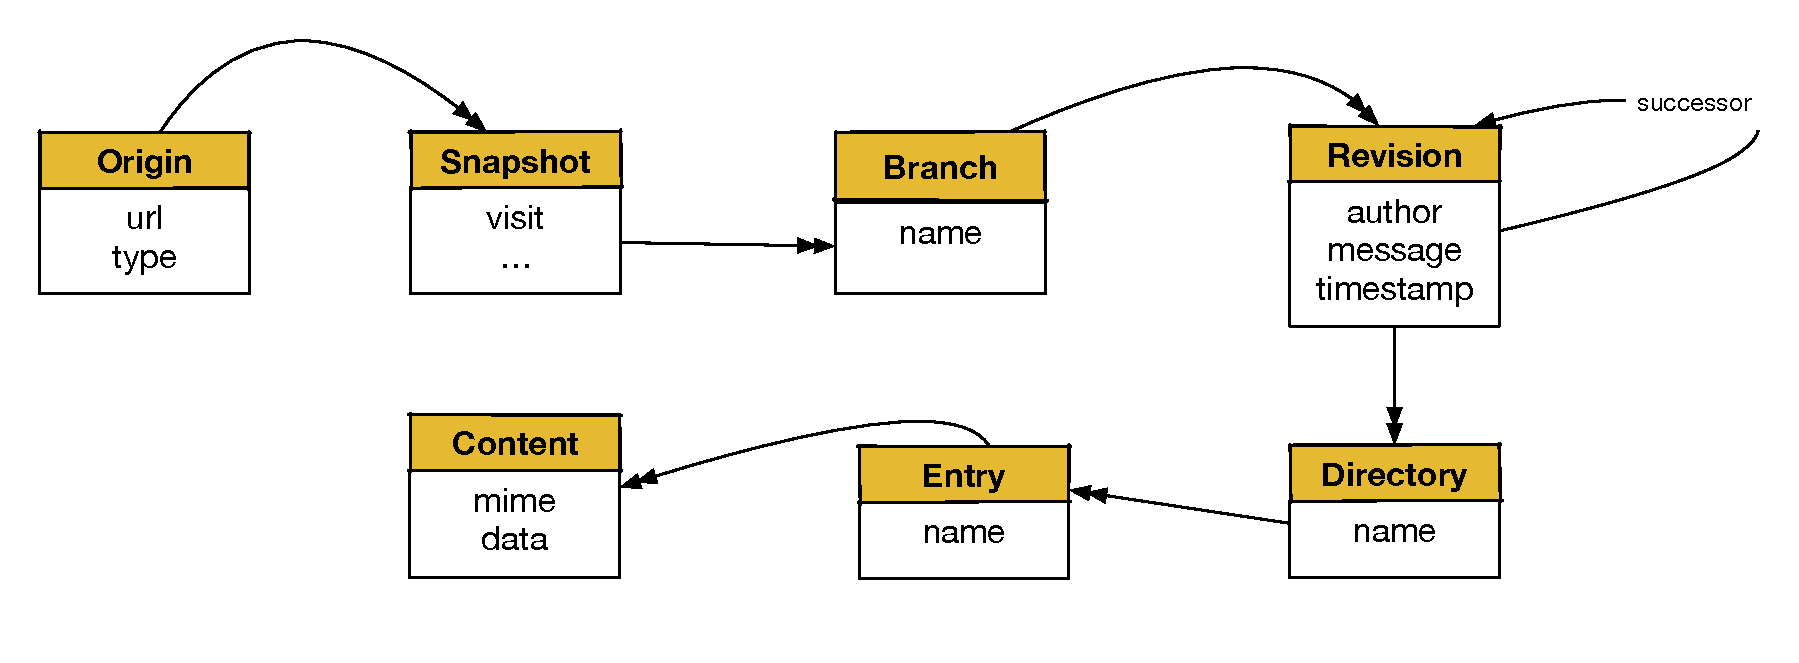
\includegraphics[height=.6\textheight]{../figures/modele_swh.pdf}
\end{center}
\end{frame}


%%%%%%%%%%%%%
\begin{frame}[fragile] \frametitle{Commençons\,: cherchons les visites}

Une première approche purement relationnelle ne fonctionne pas.
\vfill

\begin{columns}
    \begin{column}{0.45\textwidth}
    \alert{Schema}
    \end{column}
        \begin{column}{0.45\textwidth}
    \alert{Queries}
    \end{column}
\end{columns}

\begin{columns}
    \begin{column}{0.45\textwidth}
  \begin{minted}{sql}
  create table Origin 
     (origin_id uuid,
      url varchar, 
      description text,
      primary key (origin_id))
  \end{minted}
  
  \begin{minted}{sql}
  create table Visit 
     (visit_id uuid,
      origin_id
      visit_ref int,
      date date,
       primary key (visit_id) )
  \end{minted}
  \end{column}
 \begin{column}{0.45\textwidth}
  Il faut deux requêtes (pas de jointure)
  \vfill
  \begin{minted}{sql}
  select origin_id in oid 
  from Origin 
  where url ='swh.org'
  \end{minted}

  \begin{minted}{sql}
  select * from Visit 
  where origin_id = oid
  \end{minted}
  \vfill
  Et Cassandra refuse les deux !
\end{column}
\end{columns}

\end{frame}


%%%%%%%%%%%%%
\begin{frame}[fragile] \frametitle{Mieux}

Les critères de recherche doivent être dans la clé

\vfill
\begin{columns}
    \begin{column}{0.45\textwidth}
  \begin{minted}{sql}
  create table Origin 
     (url varchar, 
      description text,
      primary key (url)
      )
  \end{minted}
  
  \begin{minted}{sql}
  create table Visit 
     (url_origin varchar,
      visit_ref int,
      date date,
      primary key (url_origin, visit_id)
      )
  \end{minted}
  \end{column}
 \begin{column}{0.45\textwidth}
  Une requête localisée et séquentielle
  \vfill

  \begin{minted}{sql}
  select * from Visit 
  where  url ='swh.org'
  \end{minted}
  
\end{column}
\end{columns}

\end{frame}
	
	
%%%%%%%%%%%%%
\begin{frame}[fragile] \frametitle{Avec dénormalisation}

\vfill
\begin{columns}
    \begin{column}{0.45\textwidth}
    
    Un type \texttt{Visit}
    
  \begin{minted}{sql}
  create type Visit (
      number int,
      date_visit date)
  \end{minted}
    
    \vfill
    Imbriqué dans \texttt{Origin}
    \vfill
  \begin{minted}{sql}
  create table Origin 
     (url varchar, 
      description text,
      visites list<Visit>,
      primary key (url)
      )
  \end{minted}
  
  \vfill
  Suppose un nombre limité de visites.
   \end{column}
 \begin{column}{0.45\textwidth}
  Une requête localisée et unique pour trouver toutes les visites d'une origine.

  \begin{minted}{sql}
  select * from Origin 
  where  url ='swh.org'
  \end{minted}
  
  \vfill
  La seconde visite
  
   \begin{minted}{sql}
  select * from Origin 
  where  url ='swh.org'
  and visit.number=2
  \end{minted}
  
\end{column}
\end{columns}
	
\end{frame}


%%%%%%%%%%%%%
\begin{frame}[fragile] \frametitle{En privilégiant l'accès \texttt{Origin} $\to$ \texttt{Snapshot}}


\begin{columns}
    \begin{column}{0.45\textwidth}
     
  \begin{minted}{sql}
  create type Origin (
      description int,
      other_infos text)
  \end{minted}
    
    \vfill
  \begin{minted}{sql}
  create table Snapshot 
     (url varchar, 
      snapshot_date,
      snapshot_id uuid,
      origin Origin,
      visits map<date, Visit>,
      branches list<string>,
      primary key (url, snapshot_date)
      )
  \end{minted}
  
  \vfill
  Suppose un nombre limité de visites et de branches
   \end{column}
 \begin{column}{0.45\textwidth}
  Tous les snapshots d'une origine.
  
  \vfill
  
  \begin{minted}{sql}
  select * from Snapshot 
  where  url ='swh.org'
  \end{minted}
  
   \vfill
   Snapshots après une date et contenant une branche \texttt{master}
   
 \begin{minted}{sql}
  select * from Snapshot 
  where  url ='swh.org'
  and snapshot_date > '01-MARCH-2024'
  and branches contains key 'master'
  \end{minted}

\end{column}
\end{columns}
	
\end{frame}
	
	
%%%%%%%%%%%%%
\begin{frame}[fragile] \frametitle{Exemples pour \texttt{Revision}, \texttt{Directory}, \texttt{Entry}}


\begin{columns}
    \begin{column}{0.45\textwidth}
   Ici, vraie sructure de graphe. À creuser, car autant
   de requêtes que d'ancêtres\ldots
   
  \begin{minted}{sql}
  create table Revision 
     (branch_id uuid, 
      revision_id uuid,
      parent_id uuid,
      author varchar,
      message varchar,
      timestamp date, 
      primary key (branch_id, revision_id)
      )
  \end{minted}
  
  
   \end{column}
 \begin{column}{0.45\textwidth}
 
\end{column}
\end{columns}
	
\end{frame}
	
\end{document}


	
\begin{frame}[fragile]{Clause $WHERE$}
\begin{itemize}
	\item \textbf{Clé primaire = valeur} : Le plus efficace
	\item \textbf{token(Clé primaire) $>$ valeur} : Liste de tokens par noeud
	\item \textbf{attribut = valeur} + \textbf{INDEX} : Moins efficace
	\item \textbf{attribut = valeur} + \textbf{ALLOW FILTERING} : Pas efficace\\test sur tous les noeuds
	\item \textbf{Données imbriquées} :
	\begin{itemize}
		\item \textsc{SET} : \textit{CONTAINS}
		\item \textsc{LIST} : \textit{CONTAINS}
		\item \textsc{MAP} : \textit{CONTAINS KEY}\\ou clé directement : hotesse.prenom = 'Natacha'\\
		Les clés peuvent être indexées
		\item \textsc{SubType} : att = valeur (tuple imbriquée = BLOB)
		\item[$\Rightarrow$] Le \textit{MAP} est à privilégier
	\end{itemize}
\end{itemize}
\end{frame}

\end{document}